\documentclass[conference]{IEEEtran}
\usepackage{graphicx}
\usepackage{amsmath}

\begin{document}
\title{A hypothetical approach towards traveling in space in absence of Time}
\author
{\IEEEauthorblockN{NIKHIL DHANDRE}
\IEEEauthorblockA{SCOE, Pune}}
\maketitle
\section{Travelling in absence of time}
Consider a cuboid is .
\begin{figure}[htbp]
\centering
		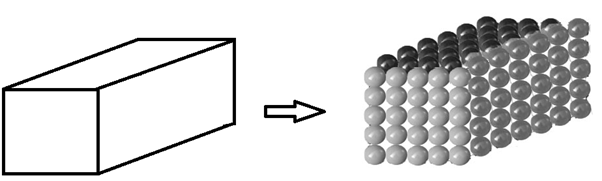
\includegraphics[scale=0.5]{img1.png}
\end{figure}
Consider each marble ball as the space-time which is covering the space three dimentionally. Now watch the arrangement of the marbles:
\begin{enumerate}
\item	Each ball 
\item	The balls 
\begin{figure}[htbp]
	\centering
		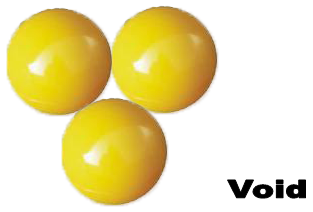
\includegraphics[scale=0.5]{img2.png}
\end{figure}
\item	As the void is remaining as unoccupied space and one more thing one can move from one void to other because voide of time i.e. relative time.
\begin{itemize}
\item	This makes toesn't contain relative time.
\end{itemize}
\section{Theory supports existence of Black Hole}
``An elementary But even then mass and other calculations of black hole are done as:
$$ M^{~}(C^2/G)^{3/2}\rho^{-1/2} $$
Where,\\ $M =$ Mass
	$G =$ Gravity,
	$\rho =$ Density,
	$C =$ speed of light in vacuum.\\
	
time atom. \\
\begin{itemize}
\item 	Point supporting
\begin{itemize}
\item	The nearer 
\item	As the relative time \\
\begin{figure}[htbp]
	\centering
		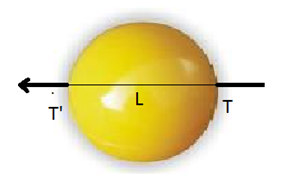
\includegraphics[scale=0.5]{img3.png}
\end{figure}
As relative time is zero. So,
$$ T=T'\, $$
\item	As there le be just a void so there may be possibility of transmitting of x-rays too.
\end{itemize}
\item	Contradictory points
\begin{itemize}
\item	It doesn'
\item	Also ther
\end{itemize}
\end{itemize}
\end{enumerate}
\section{Merits}
\begin{itemize}
\item	If we wil
\item	May be sul to light.
\end{itemize}

\section{Limitations}
Such voids are 

\section{Conclusion}
Such theories  must also be checked and to be taken as a new theory on the way of exploring wonders of the universe.
\begin{thebibliography}{9}
\bibitem{it1}	Patrick Moore, \emph{Our Universe: An Introduction}
ISBN 13 : 978104332411
\bibitem{it2} University Science Books,	\emph{The Physical Universe An Introduction to Astronomy}
ISBN: 0-935702-05-9
\bibitem{it3}	Dravyanuyoga- Ariyika Gyanmati, \emph{Jaina bharati(Jainism scripture): the essence of Jainism-Section 4}
\bibitem{it4}	\emph{Tatvarthsutra(Jainism scripture): Chapter 5 verse 29}
\bibitem{it5}	Friedrich W. Hehl, Claus Kiefer, Ralph J.K. Metzler (Eds.), \emph{Black hole: theory and observation}
ISBN: 3-54065158-6
\bibitem{it6}	Edwin Thomas, \emph{Black Hole: An Introduction- Derek Raine}
\end{thebibliography}
\end{document}